\documentclass[10pt,a4paper]{article}
\usepackage[latin1]{inputenc}
\usepackage{amsmath}
\usepackage{amsfonts}
\usepackage{amssymb}
\usepackage{mathtools}
\usepackage{bm}
\usepackage{standalone}
\usepackage{graphicx}
\usepackage{float}
% Use \bm{x} for vectors/matrices in bold AND italic

\begin{document}

\section*{Single Source In Unit Box}
In this simple example we model a single source located in the origin of a unit box with Dirichlet boundary conditions. In this solution we have used 1000 points in each spatial direction. A grid as fine as this shows very clearly the source in form of a spire located in the origin. We can also see the symmetry of the solution.

\begin{figure}[H]
\centering
    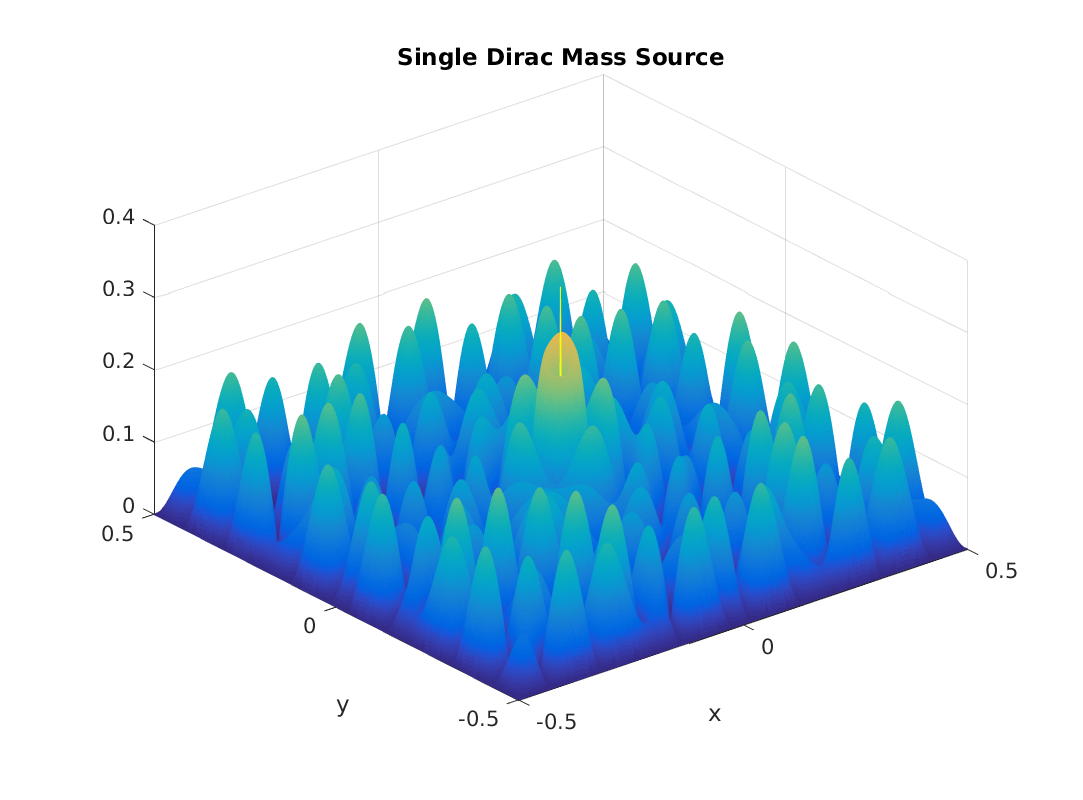
\includegraphics[width=0.9\textwidth]{figures/SingleSource_2D_1000.eps}
	\caption{A single source in unit box with Dirichlet boundary conditions.}
  \label{fig:singleSource1000}
\end{figure}

\end{document}